\chapter{Etude préalable}

\section{Introduction}

Ce premier chapitre permet de placer le projet dans son contexte général. Il commence par une présentation de l’entreprise MEDIANET, dans lequel le projet a été mené, puis introduit le projet, son contexte ainsi que ses objectifs principaux.

\section{Présentation de l'organisme d'accueil}

\textbf{MEDIANET} est une agence IT, marketing digital et conseil stratégique AI-first, spécialisée dans la transformation digitale.

Depuis plus de 25 ans, elle accompagne les entreprises, institutions et gouvernements dans la conception, le développement et la croissance de leurs activités grâce à une approche combinant technologie, data, marketing digital et intelligence artificielle.

Avec plus de vingt ans d’expérience dans le développement web, les applications mobiles et le marketing digital, MEDIANET aide les organisations à se transformer numériquement en leur proposant des solutions complètes et adaptées à leurs besoins. Grâce à son approche globale, elle peut proposer un accompagnement couvrant toutes les étapes de la digitalisation.

\begin{figure}[H]
    \centering
        
\includegraphics[width=0.8\textwidth]{images/autre/logo-medianet.png}
    \caption{Logo de l'entreprise MEDIANET}
    \label{fig:logo}
    \small source : \parencite{medianet_2026}
\end{figure}



\subsection{Vision et mission}

\noindent
\textbf{Vision :} Développer un écosystème basé sur le co-leadership, composé d'experts créatifs et socialement responsables, favorisant et renforçant l'innovation et la transformation technologique.

\noindent
\textbf{Mission :} Créer, développer et optimiser le business des entreprises à l’international en utilisant la technologie et la créativité.

\subsection{Engagements qualité}

MEDIANET adopte un système de gestion de la qualité en adéquation avec les exigences de la norme ISO 9001 et s'investit dans une démarche visant à améliorer en permanence. Ses principaux engagements sont les suivants :

\begin{itemize}
\item Améliorer de manière continue la performance des solutions développées ainsi que la qualité des livrables, en tenant compte des retours clients et en anticipant leurs attentes afin de renforcer leur satisfaction
\item Garantir une réactivité efficace dans la prise en charge des opérations de maintenance
\item Accroître le développement commercial sur les marchés nationaux et internationaux
\item Respecter les délais contractuels de réalisation des projets.
\item Adapter en permanence les programmes de formation en fonction des besoins évolutifs des clients
\end{itemize}


\subsection{Secteurs d’activités}

MEDIANET est active dans plusieurs domaines, notamment :

\begin{itemize} 
    \item E-gov
    \item Banques
    \item Assurances
    \item Tourisme
    \item E-commerce
    \item Grande Distribution
    \item Santé
    \item Automobile
    \item Transport
    \item Immobilier
    \item Industrie
\end{itemize}


\section{Contexte général du projet}
Cette partie présente le cadre du projet E-Gouv, le contexte général, la problématique relevée, les solutions existantes, ainsi que la solution proposée et ses objectifs.

\subsection{Cadre du projet}

Ce travail de fin d’études est réalisé dans le cadre de l’obtention du diplôme d’ingénieur en informatique à l’ESPRIT. Il a été fait en six mois au sein de l’entreprise MEDIANET.

\subsection{Contexte du projet}

Située au cœur du continent africain, la République Centrafricaine (RCA) s’inscrit progressivement dans une dynamique de modernisation de ses institutions et de ses services publics. Face aux mutations technologiques mondiales et aux nouvelles attentes des citoyens en matière d’accessibilité et d’efficacité administrative, le pays considère aujourd’hui la transformation numérique comme un levier stratégique de développement économique, social et institutionnel.

Cette volonté de modernisation vise notamment à renforcer la transparence administrative, améliorer la qualité des services publics et rapprocher l’administration des citoyens. Toutefois, cette transformation s’inscrit dans un contexte où les infrastructures numériques restent encore en développement et où l’accès aux technologies de l’information demeure limité pour une partie importante de la population.

Comme l’illustre le graphique ci-dessous, basé sur les données de la Banque Mondiale, le taux d’accès à Internet en République Centrafricaine demeure relativement faible, avec environ 14 \% d’utilisateurs en 2024, un niveau inférieur à celui observé dans plusieurs pays voisins. Cette situation met en évidence les défis liés à l’inclusion numérique et à l’accessibilité des services digitaux.

\begin{figure}[H]
    \centering
    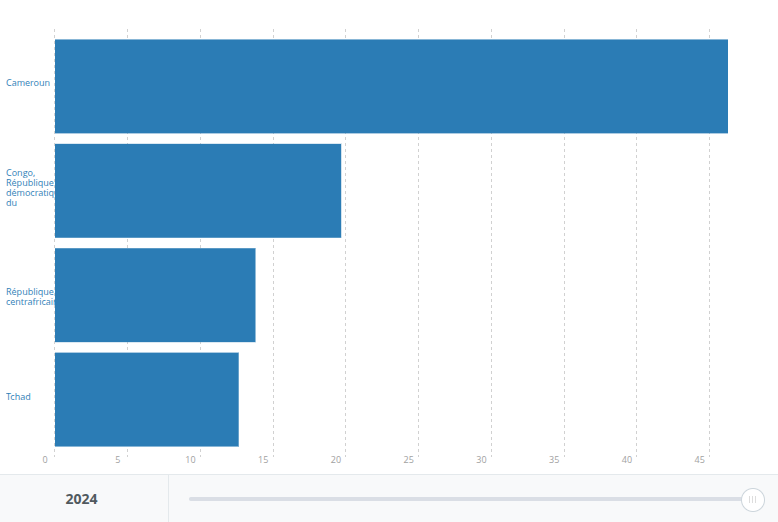
\includegraphics[width=0.8\textwidth]{images/autre/graph-population-internet.png}
    \caption{Pourcentage des utilisateurs accédant à internet - Central African Republic, Chad, Cameroon, Congo, Dem. Rep.}
    \label{fig:worldbank}
\end{figure}


Malgré ces contraintes, ce contexte souligne également l’importance stratégique de la digitalisation des services publics comme moteur d’amélioration administrative. En effet, la mise en place de solutions numériques adaptées permettrait d’accélérer le traitement des démarches administratives, de simplifier les procédures, de renforcer la traçabilité des demandes et d’améliorer la communication entre les institutions publiques et les citoyens, y compris dans des environnements caractérisés par des contraintes infrastructurelles importantes.

C’est dans cette perspective qu’intervient notre projet \textbf{e-Gouv}, fondé sur le concept de la \textbf{gouvernance électronique} (\textit{e-Government}). Cette approche consiste à intégrer les technologies numériques dans les processus administratifs afin d’optimiser la gestion publique, améliorer la qualité des services offerts et favoriser une administration plus accessible, transparente et efficace.

Le concept de gouvernance électronique s’appuie sur quatre piliers de base :

\begin{itemize}
    \item \textbf{Les ressources} : elles comprennent l’ensemble des infrastructures, des moyens organisationnels et des données nécessaires au bon fonctionnement du système d’information gouvernemental.

    \item \textbf{La technologie} : elle représente les solutions numériques et les outils technologiques mobilisés pour concevoir une plateforme moderne, sécurisée, performante et accessible.

    \item \textbf{Les processus} : ce pilier concerne l’optimisation, la simplification et la digitalisation des procédures administratives afin d’améliorer l’efficacité des opérations et de réduire les délais de traitement.

    \item \textbf{Les personnes} : elles représentent les acteurs impliqués dans le système, y compris les administrations publiques, les responsables institutionnels, les agents administratifs et les citoyens bénéficiaires des services.
\end{itemize}

Ainsi, le projet \textbf{e-Gouv} s’inscrit dans une démarche de modernisation de l’administration publique centrafricaine en proposant une plateforme numérique centralisée capable de faciliter l’accès aux services administratifs, d’améliorer leur gestion et de renforcer l’interaction entre l’État et les citoyens.



\subsection{Problématique}

Malgré les efforts entrepris par la République Centrafricaine pour moderniser son administration publique, la gestion des services administratifs reste confrontée à plusieurs limites qui freinent encore son efficacité globale.

Dans de nombreux cas, les démarches administratives reposent encore sur des processus manuels et l’utilisation de documents papier. Cette situation entraîne non seulement des délais de traitement relativement longs, mais également une consommation importante de ressources et un risque non négligeable d’erreurs ou de perte d’information.

Par ailleurs, l’absence d’une plateforme unifiée regroupant l’ensemble des services publics conduit à une fragmentation des systèmes d’information. Chaque administration utilise souvent ses propres outils, ce qui limite l’interopérabilité, complique le partage des données et réduit la coordination entre les différents acteurs institutionnels.

En outre, le suivi des demandes administratives reste peu transparent pour les citoyens. Ces derniers disposent rarement d’une visibilité claire et en temps réel sur l’état d’avancement de leurs dossiers, ce qui les oblige fréquemment à se déplacer physiquement auprès des services concernés.

Enfin, le niveau limité de digitalisation, notamment l’absence d’outils intelligents d’assistance aux usagers, rend l’accès à l’information administrative plus difficile, en particulier pour les citoyens peu familiers avec les procédures administratives.

Ces contraintes ont des impacts directs sur le fonctionnement global de l’administration, notamment :
\begin{itemize}
    \item l’allongement des délais de traitement des démarches
    \item la dégradation de la qualité de service perçue par les usagers
    \item l’absence de transparence dans le suivi des dossiers
     \item une gestion globale inefficace des ressources administratives
\end{itemize}

Dans ce contexte, il apparaît nécessaire de concevoir une solution numérique intégrée, capable de centraliser les services publics, de renforcer la coordination entre les administrations et d’améliorer de manière significative l’accessibilité ainsi que la transparence des services offerts aux citoyens.











\subsection{Etude de l'existant : Benchmark des plateformes de référence}

Afin d’identifier les bonnes pratiques en matière de digitalisation des services publics et d’orienter la conception de la solution proposée, une étude comparative de plateformes de référence a été réalisée. Cette analyse se concentre sur des solutions reconnues à l’échelle internationale, illustrant différents aspects clés tels que la sécurité, l’inclusion numérique et la gestion à grande échelle des services publics.

\subsubsection{FranceConnect (France)}
 


\begin{figure}[H]
\centering
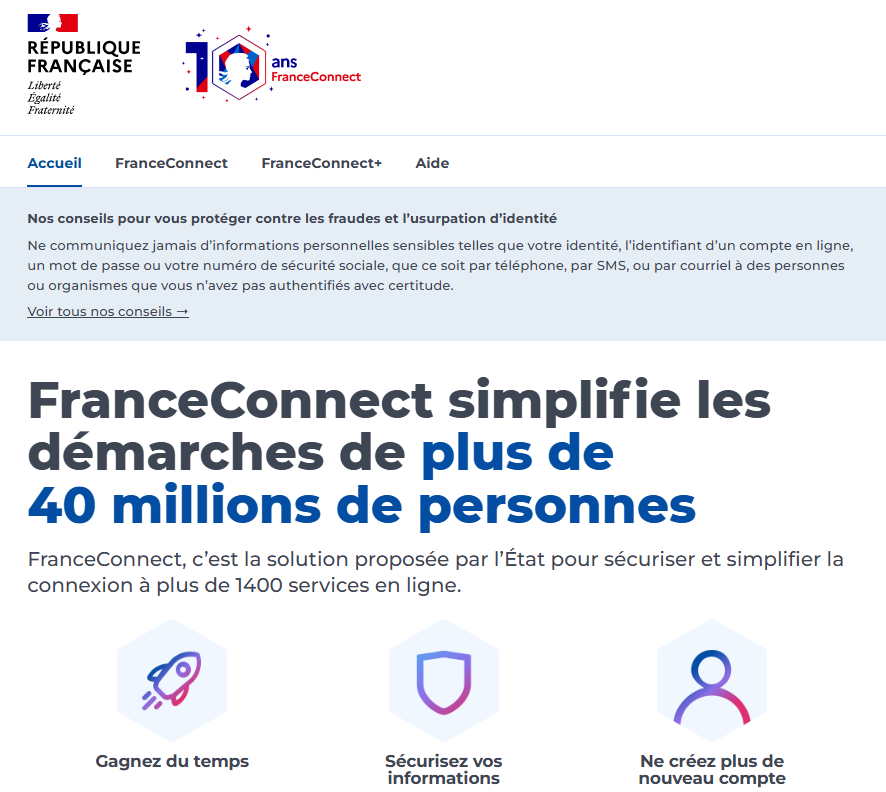
\includegraphics[width=0.8\textwidth]{images/autre/FranceConnect.png}
\caption{Le Système FranceConnect}
\label{fig:franceconnect}
\end{figure}



FranceConnect est un système d’identité numérique unifiée permettant aux citoyens d’accéder à un large ensemble de services publics en ligne à l’aide d’un seul compte sécurisé. Il constitue une référence en matière de fédération d’identités et de sécurité des accès. Le tableau \ref{tab:franceconnect} présente une analyse des points forts et faibles de la plateforme FranceConnect.

\begin{table}[H]
\centering

% lignes alternées
\rowcolors{2}{gray!15}{white}

% bordures fines
\setlength{\arrayrulewidth}{0.3pt}

\begin{tabular}{|p{0.45\textwidth}|p{0.45\textwidth}|}
\hline
\rowcolor{gray!30}
\textbf{Points Forts} & \textbf{Points Faibles} \\
\hline

 
\begin{itemize}
    \item Interopérabilité maximale entre plus de 1000 services publics
    \item Sécurité renforcée avec authentification à deux facteurs
\end{itemize}
 
&
 
 
\begin{itemize}
    \item Interfaçage complexe, ce qui implique une difficulté d’utilisation pour certains usagers \parencite{franceconnect_gaps}
\end{itemize}
 
\\
\hline

\end{tabular}

\caption{Analyse de la plateforme FranceConnect}
\label{tab:franceconnect}
\end{table}

\subsubsection{IremboGov (Rwanda)}
 


\begin{figure}[H]
\centering
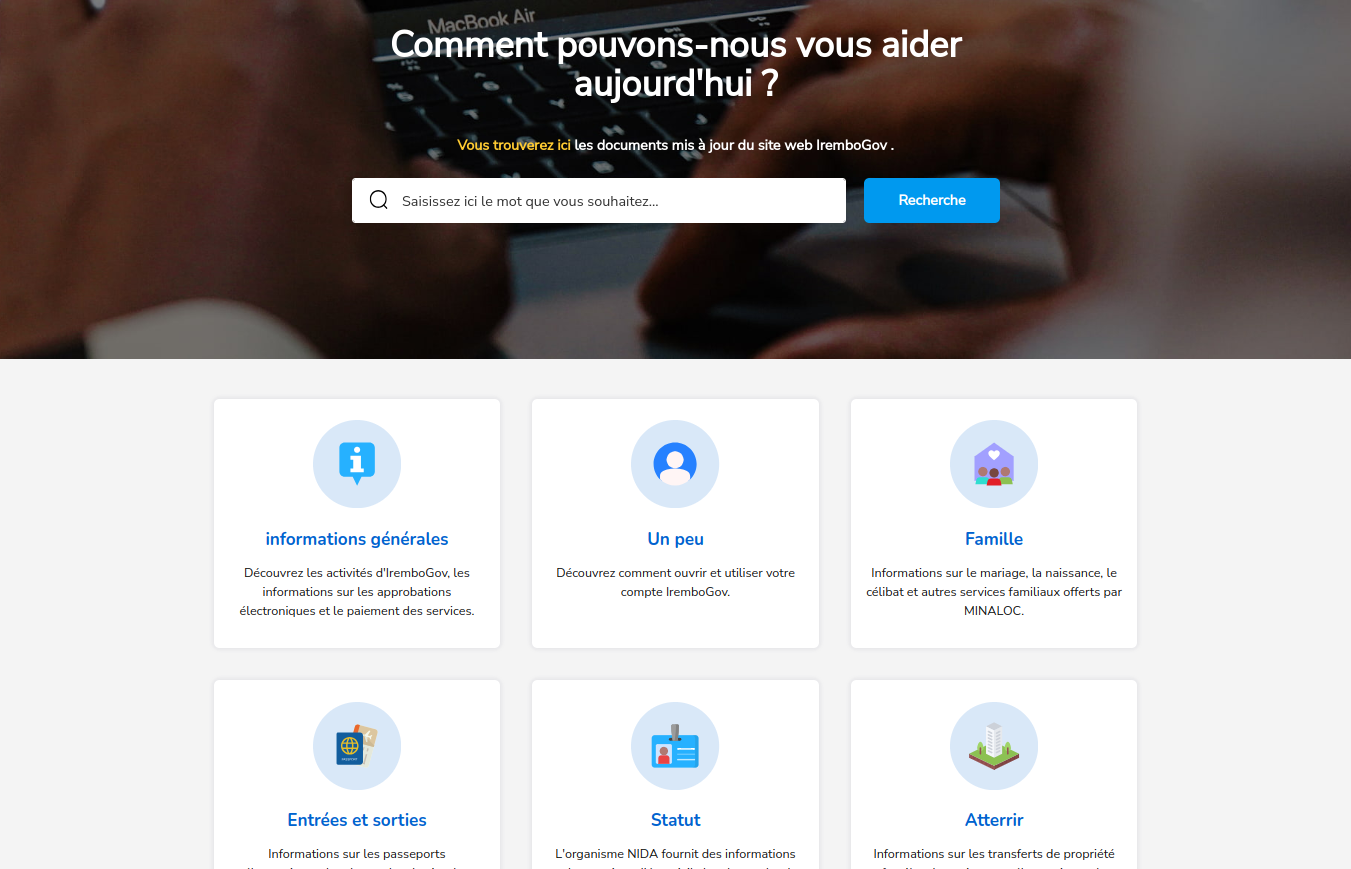
\includegraphics[width=0.8\textwidth]{images/autre/irembo.png}
\caption{La Plateforme IremboGov}
\label{fig:irembo}
\end{figure}









 
IremboGov est une plateforme nationale rwandaise de services publics en ligne, conçue pour répondre aux contraintes spécifiques du contexte africain. Elle permet aux citoyens d’accéder à de nombreux services administratifs via des canaux numériques et hybrides.
 Le tableau \ref{tab:irembo_analysis} présente l'analyse de la plateforme IremboGov.
\begin{table}[H]
\centering

% lignes alternées gris/blanc
\rowcolors{2}{gray!15}{white}

% bordures fines
\setlength{\arrayrulewidth}{0.3pt}

\begin{tabular}{|p{0.45\textwidth}|p{0.45\textwidth}|}
\hline
\rowcolor{gray!30}
\textbf{Points Forts} & \textbf{Points Faibles} \\
\hline

 
\begin{itemize}
    \item Forte adaptation au contexte africain
    \item Intégration de moyens de paiement locaux
\end{itemize}
 
&
 
\begin{itemize}
    \item Des problèmes techniques perturbent parfois la disponibilité du service
    \item Les déplacements des citoyens vers l’administration sont encore nécessaires pour compléter certaines démarches \parencite{rwanda_e_gov_gaps}
\end{itemize}
 
\\
\hline

\end{tabular}

\caption{Analyse de la plateforme IremboGov}
\label{tab:irembo_analysis}
\end{table}

\subsubsection{Ghana.gov (Ghana)}
 


\begin{figure}[H]
\centering
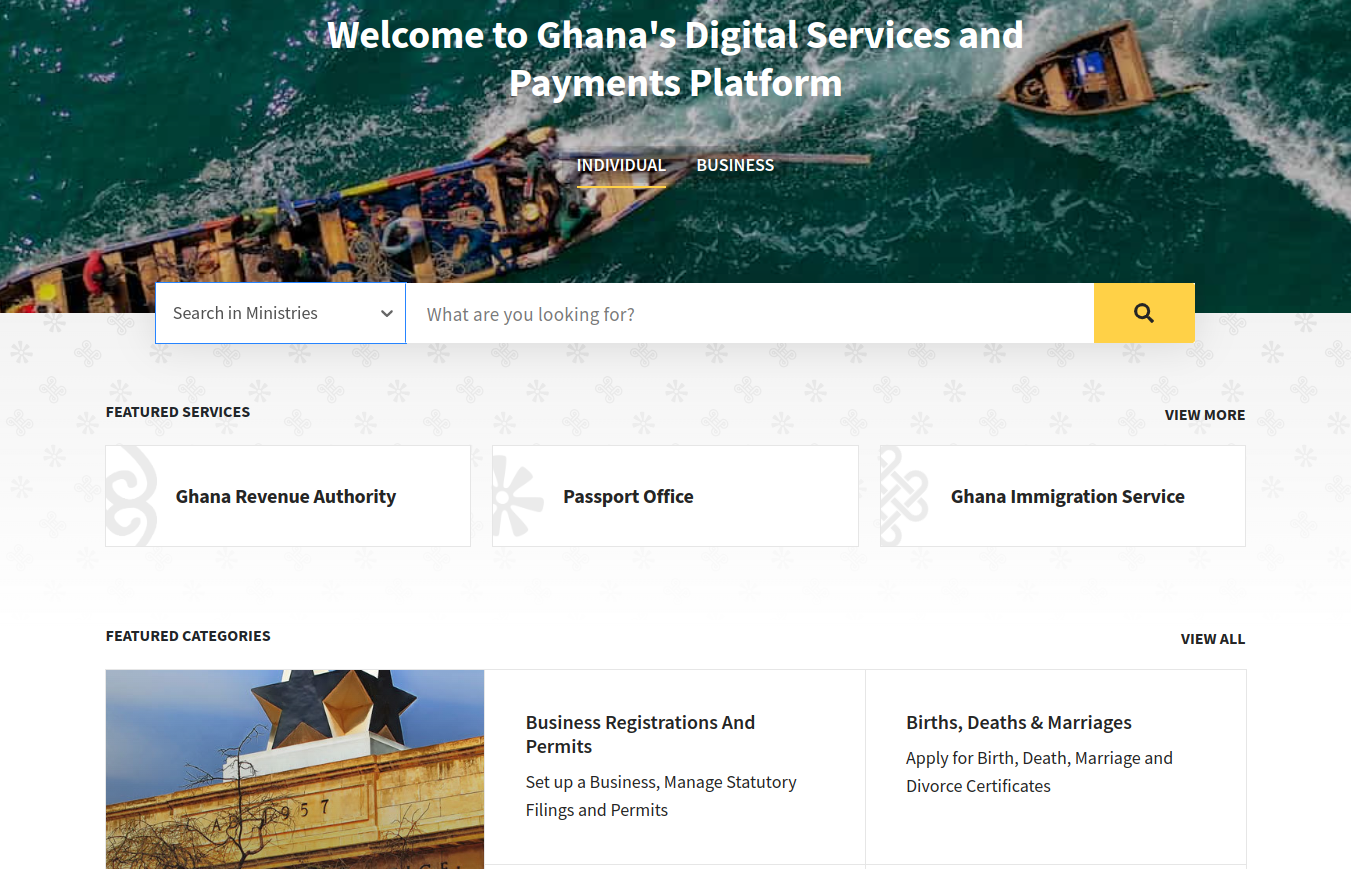
\includegraphics[width=0.8\textwidth]{images/autre/ghana_gov.png}
\caption{Plateforme Ghana.gov}
\label{fig:ghanagov}
\end{figure}











Ghana.gov est le portail national des services publics numériques du Ghana. Il centralise l’accès à de nombreux services administratifs et transactionnels, en mettant l’accent sur la simplification des démarches, la transparence administrative et la digitalisation des paiements publics.  Le tableau \ref{tab:ghana_analysis} présente l'analyse de la plateforme Ghana.gov.

\begin{table}[H]
\centering

% lignes alternées gris/blanc
\rowcolors{2}{gray!15}{white}

% bordures fines
\setlength{\arrayrulewidth}{0.3pt}

\begin{tabular}{|p{0.45\textwidth}|p{0.45\textwidth}|}
\hline
\rowcolor{gray!30}
\textbf{Points Forts} & \textbf{Points Faibles} \\
\hline

 
\begin{itemize}
    \item Amélioration de la transparence et de la traçabilité des demandes
    \item Approche orientée vers la simplification des parcours citoyens
\end{itemize}
 
&
 
\begin{itemize}
    \item Stabilité du système : peut parfois souffrir de ralentissements lors des pics de demandes \parencite{ghana_portal_gaps}
\end{itemize}
 
\\
\hline

\end{tabular}

\caption{Analyse de la plateforme Ghana.gov}
\label{tab:ghana_analysis}
\end{table}




\subsubsection{Synthèse comparative des plateformes étudiées}

Le tableau \ref{tab:benchmark_synthese} présente une synthèse selon plusieurs critères essentiels liés à la gouvernance électronique.

\rowcolors{2}{gray!15}{white}
\setlength{\arrayrulewidth}{0.3pt}

\begin{longtable}{|p{3.5cm}|p{3.5cm}|p{3.5cm}|p{3.5cm}|}

\hline
\rowcolor{gray!30}
\textbf{Critères} & \textbf{FranceConnect} & \textbf{IremboGov} & \textbf{Ghana.gov} \\
\hline
\endfirsthead

\hline
\rowcolor{gray!30}
\textbf{Critères} & \textbf{FranceConnect} & \textbf{IremboGov} & \textbf{Ghana.gov} \\
\hline
\endhead

Type de plateforme & Fédération d’identité & Portail de services publics & Portail national e-gov \\
\hline

Cible principale & Citoyens / administrations & Citoyens (contexte africain) & Citoyens / entreprises \\
\hline

Niveau de centralisation & Très élevé & Moyen à élevé & Élevé \\
\hline

Interopérabilité & Très forte & Moyenne & Bonne \\
\hline

Accessibilité numérique & Élevée & Adaptée au contexte local & Élevée mais dépendante de l’infrastructure \\
\hline

Services transactionnels & Limité (authentification) & Oui & Oui \\
\hline

Adaptation au contexte africain & Faible & Très forte & Moyenne \\
\hline

Limites principales & Complexité d’intégration & Instabilité technique & Ralentissements en charge \\
\hline
\rowcolor{white}
\caption{Synthèse comparative des plateformes de gouvernance électronique}
\label{tab:benchmark_synthese}

\end{longtable}


















\subsection{Solution proposée}

Pour répondre aux objectifs liés à la modernisation et à la transformation numérique des services publics en RCA, ce projet propose la conception et la mise en œuvre d’une \textbf{plateforme web sécurisée et évolutive}. Celle-ci a pour vocation d’améliorer la qualité des services administratifs, de renforcer la coordination entre les différentes administrations et de simplifier l’accès des citoyens aux démarches en ligne.

La plateforme permet :

\begin{itemize}
    \item aux administrations de structurer, configurer et gérer leurs services de manière dynamique, incluant le traitement, le suivi et l’archivage des demandes et des réclamations ;
    \item aux responsables administratifs de superviser les activités opérationnelles, de suivre l’avancement des demandes, d’analyser les indicateurs statistiques et de coordonner les équipes et les services ;
    \item aux citoyens de déposer, suivre et évaluer leurs démarches administratives en ligne, de consulter les notifications et d’accéder de manière simplifiée aux informations relatives aux services publics ;
    \item d’assister les citoyens grâce à un assistant conversationnel intelligent, fondé sur l’intelligence artificielle générative et une approche RAG (génération augmentée par la recherche), qui répond en langage naturel à leurs questions et oriente vers une assistance humaine en cas de besoin.
\end{itemize}

La solution repose sur trois espaces :

\begin{itemize}
    \item \textbf{Portail} : Point d’accès public et centralisé aux services dématérialisés. Il permet la consultation des actualités, des projets institutionnels, des informations générales ainsi que la liste des ministères et de leurs responsables. Hautement paramétrable, ce portail offre aux administrateurs la possibilité de gérer dynamiquement les contenus et les informations diffusées. Il intègre également un assistant conversationnel intelligent qui répond aux questions des citoyens en langage naturel.
    \item \textbf{Backoffice Administrateur} : Un espace dédié aux administrateurs de la plateforme pour gérer les tâches. Il permet de personnaliser les services, d'assigner des rôles aux utilisateurs, de définir les processus de traitement, ainsi que de superviser l'ensemble du système.
    \item \textbf{Espace Client} : Espace personnel dédié aux citoyens, leur permettant de déposer et suivre leurs demandes de services, de consulter l’état de traitement de leurs réclamations, de recevoir des notifications et de gérer les paramètres de leur compte.
\end{itemize}

Cette solution permet ainsi de \textbf{centraliser, moderniser et sécuriser} la gestion des services administratifs, tout en assurant une expérience utilisateur fluide, cohérente et adaptée aux besoins des différents acteurs du système.


\section{Les méthodologies de gestion de projet}

La gestion de projet permet d’organiser les activités, de structurer les responsabilités, de maîtriser les délais et d’assurer une coordination efficace entre les différentes parties prenantes. Dans le domaine du génie logiciel, plusieurs méthodologies de gestion de projet sont utilisées. Elles se répartissent généralement en deux grandes familles : les approches prédictives (traditionnelles) et les approches adaptatives (agiles) \parencite{pmbok2017} .
 

\subsection{Méthodologies traditionnelles (prédictives)}

Les méthodologies traditionnelles, souvent qualifiées d’approches prédictives, s’appuient sur une planification exhaustive réalisée en amont du projet. Elles reposent sur une organisation séquentielle et rigoureuse, où chaque phase doit être complétée avant d’aborder la suivante. Ce type d’approche est généralement privilégié lorsque les exigences sont clairement définies et stables dès le lancement du projet \parencite{pressman2014}.

Parmi ces méthodes, le modèle en cascade (\textit{Waterfall}) figure parmi les plus répandus. Il organise le cycle de vie du projet en une succession d’étapes distinctes, allant de l’analyse des besoins à la maintenance, en passant par la conception, le développement, les tests et le déploiement. Cette approche se distingue par une forte traçabilité documentaire et une vision globale bien structurée du projet. Néanmoins, sa rigidité constitue une limite importante, notamment face aux évolutions des besoins, et l’intégration tardive des retours utilisateurs peut réduire l’adéquation du produit final aux attentes réelles \parencite{sommerville2016}.


\subsection{Méthodologies agiles (adaptatives)}

Les méthodologies agiles ont été introduites pour répondre aux limites des approches prédictives, notamment dans les environnements où les besoins évoluent rapidement. Elles reposent sur une démarche itérative et incrémentale. Ce derniers permet une adaptation continue ainsi qu’une amélioration progressive du produit \parencite{agilemanifesto}.

Ces méthodes se concentrent sur la collaboration étroite entre les membres de l'équipe, sur l'engagement constant du client et sur la livraison fréquente des versions fonctionnelles du système. Cette organisation permet de diminuer les risques liés aux changements d’exigences et d’améliorer de façon progressive la qualité du produit livré.

Scrum, Kanban et Extreme Programming (XP) sont parmi les méthodes agiles les plus employées. Scrum convient particulièrement bien aux projets complexes qui nécessitent une forte interaction avec le client et une organisation du travail en cycles courts, appelés \textit{Sprints} \parencite{schwaber2020}. Kanban met l’accent sur la visualisation du flux de travail et sur l’amélioration continue, tandis que XP se concentre sur les bonnes pratiques de développement logiciel.



 













 
\subsection{Synthése des methodologies de gestion de projet}

Comme présenté dans le tableau \autoref{tab:synthese-methodologies}, les approches agiles et prédictives diffèrent sur plusieurs aspects essentiels.

\rowcolors{2}{gray!15}{white}
\setlength{\arrayrulewidth}{0.3pt}
\begin{longtable}{|p{3cm}|p{5.5cm}|p{5.5cm}|}
\hline
\rowcolor{gray!30}
\textbf{Aspect} & \textbf{Approches prédictives} & \textbf{Approches agiles} \\ \hline
\endfirsthead

 

Principe &
Planification complète et détaillée en amont du projet &
Approche itérative et incrémentale basée sur l’adaptation continue \\ \hline

Organisation &
Processus séquentiel structuré en phases successives &
Cycles courts appelés itérations ou Sprints \\ \hline

Flexibilité &
Peu de flexibilité pour faire face aux changements &
Une grande capacité à s'adapter aux évolutions \\ \hline

Implication du client &
Une intervention au début et à la fin du projet &
Un engagement continu pendant toute la durée du projet \\ \hline

Livraison &
Livraison finale unique en fin de projet &
Livraisons fréquentes de versions fonctionnelles \\ \hline

Avantages &
Structure claire, documentation complète, meilleure prévisibilité &
Réactivité, adaptation rapide, amélioration continue \\ \hline

Limites &
Rigidité et difficulté à intégrer les changements &
Moins de visibilité globale à long terme \\ \hline

Exemples &
Waterfall &
Extreme Programming (XP), Scrum, Kanban  \\ \hline
\rowcolor{white}
\caption{Synthèse des méthodologies de gestion de projet}
\label{tab:synthese-methodologies}
\end{longtable}





% tableau

\subsection{Méthode adoptée : Scrum}

La méthode Scrum a été retenue en raison de son approche itérative et incrémentale, de sa flexibilité et de sa capacité à gérer efficacement les changements de priorités. Elle permet en outre d’assurer un suivi régulier du projet et d’adapter progressivement les livrables aux besoins des utilisateurs.

Scrum se distingue par plusieurs caractéristiques essentielles :
\begin{itemize}
    \item \textbf{Détection et gestion proactive des changements} : adaptation continue aux évolutions techniques, fonctionnelles et réglementaires.
    
    \item \textbf{Responsabilisation et autonomie des équipes} : les équipes s’auto-organisent tout en restant alignées avec les objectifs du projet.
    
    \item \textbf{Approche itérative et incrémentale} : la structure du travail repose sur des cycles de 2 à 4 semaines, ce qui permet des livraisons régulières et une révision continue des priorités.
    
    \item \textbf{Transparence et inspectabilité} : l’avancement du projet, les obstacles et les décisions sont visibles par l’ensemble des parties prenantes.
\end{itemize}

La figure ci-dessous \ref{fig:scrum} illustre Le cadre Scrum.

\begin{figure}[H]
\centering
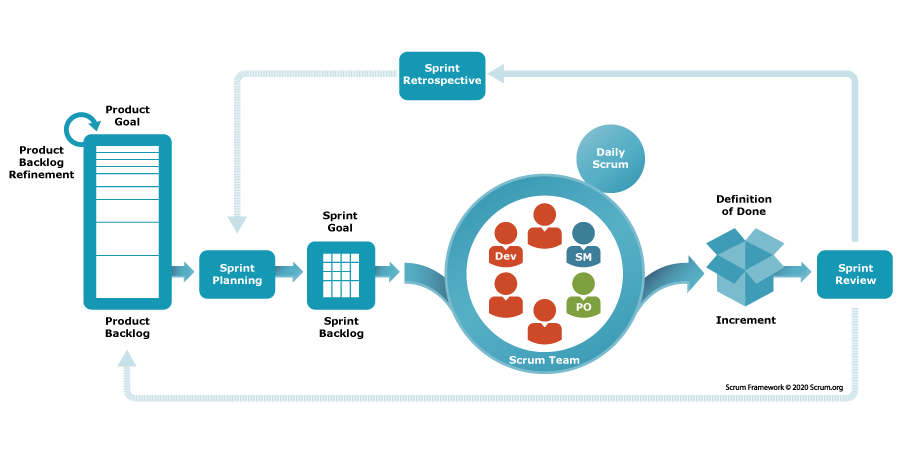
\includegraphics[width=0.9\textwidth]{images/autre/scrum.png}
\caption{Schéma du cadre Scrum}
\label{fig:scrum}
\vspace{1ex}
{\small Source : \parencite{scrum}}
\end{figure}










Chaque sprint repose sur un objectif précis et mesurable, appelé Sprint Goal, consigné dans le Sprint Backlog. Ce dernier constitue un outil de planification regroupant les tâches à exécuter, les critères d’acceptation associés, les estimations d’effort ainsi que la répartition des responsabilités entre les membres de l’équipe.

Chaque sprint s'articule autour d'un objectif clairement défini et mesurable, le Sprint Goal, qui figure dans le Sprint Backlog. Ce dernier sert de support de planification, réunissant les tâches à accomplir, les critères permettant de juger de leur bonne exécution, l'effort estimé ainsi que la répartition des rôles au sein de l'équipe.

\underline{Rituels Scrum appliqués} :

\begin{table}[h]
\centering
\begin{tabular}{|p{4cm}|p{10cm}|}
\hline
\textbf{Rituel} & \textbf{Description} \\ \hline
Réunion quotidienne (Daily Meeting) & Point rapide d'environ 15 minutes durant lequel l'équipe fait le point sur l'avancement des tâches et signale les blocages rencontrés. \\ \hline
Planification de sprint (Sprint Planning) & Rencontre organisée en amont de chaque sprint, réunissant toute l'équipe Scrum pour fixer les objectifs à atteindre et choisir les éléments du Product Backlog à traiter. \\ \hline
Revue de sprint (Sprint Review) & Moment consacré à la présentation de l'incrément produit aux parties prenantes, en vue de recueillir leurs retours et d'obtenir leur validation. \\ \hline
Rétrospective de sprint (Sprint Retrospective) & Séance d'analyse du fonctionnement de l'équipe, destinée à repérer des axes d'amélioration pour les sprints à venir. \\ \hline
\end{tabular}
\caption{Rituels Scrum appliqués}
\end{table}

\newpage
\underline{Artefacts de gestion} :

\begin{table}[h]
\centering
\begin{tabular}{|p{4cm}|p{10cm}|}
\hline
\textbf{Artefact} & \textbf{Description} \\ \hline
Carnet du produit (Product Backlog) & Liste hiérarchisée de l'ensemble des fonctionnalités à développer. \\ \hline
Carnet du sprint (Sprint Backlog) & Feuille de route détaillant les tâches à mener au cours du sprint en cours. \\ \hline
Incrément (Increment) & Somme des livrables produits au terme d'un sprint, répondant aux critères de la "Definition of Done". \\ \hline
\end{tabular}
\caption{Artefacts de gestion Scrum}
\end{table}

\subsection{Modélisation UML}
La modélisation UML (Unified Modeling Language) a été retenue dans ce projet afin de représenter le système de façon structurée et cohérente. Ce langage de modélisation standard, largement utilisé en génie logiciel, permet de décrire les différents éléments d’un système informatique ainsi que les relations existantes entre eux \parencite{uml_omg}.

Le recours à UML se justifie par sa capacité à offrir une vision claire des fonctionnalités, des acteurs et des interactions du système. Cette modélisation facilite ainsi l’analyse et la compréhension du projet, tout en permettant d’anticiper certaines incohérences de conception dès les premières phases du développement, ce qui contribue à limiter les risques et les coûts liés à des corrections tardives. 

Trois types de diagrammes sont utilisés tout au long de ce rapport :

\begin{itemize}
\item \textbf{Diagramme de cas d’utilisation} : il permet de représenter les besoins fonctionnels du système pour mettre en évidence toutes les interactions entre les acteurs et celui-ci.
\item \textbf{Diagramme de classes} : il décrit l’architecture statique du système à travers les entités manipulées, leurs attributs ainsi que les relations qui les relient.
\item \textbf{Diagramme de séquence} : il illustre le comportement dynamique du système en détaillant l’enchaînement des interactions dans le cadre d’un scénario donné.
\end{itemize}


\noindent Les diagrammes de classes et de séquence détaillés sont introduits au fil des
sprints, au plus près des fonctionnalités concernées.

\subsection{Planification du projet}
% diag de gant
Le diagramme de Gantt de la figure \ref{fig:gantt} présente
l'enchaînement de ces phases dans le temps, avec la durée estimée de chaque
sprint.

 


\begin{figure}[H]
\centering
\includegraphics[width=1\textwidth]{images/autre/gant-1.drawio.png}
\caption{Diagrame de Gantt}
\label{fig:gantt}
\end{figure}


\section{Conclusion}
Ce chapitre a pour objectif de présenter le contexte général de l’entreprise d’accueil ainsi que la problématique identifiée. Il aborde également l’analyse de l’existant et la solution proposée. Enfin, la méthodologie de travail utilisée Scrum a été décrite.